% in this file I leave the figure captions outside\ caption{} because I want them
% to be formatted in the same way as the general text (double spaced and linenumbered)
\captionsetup[figure]{labelfont={sc},labelformat={default},labelsep=period,name={Figure}}

\begin{figure}[!h]
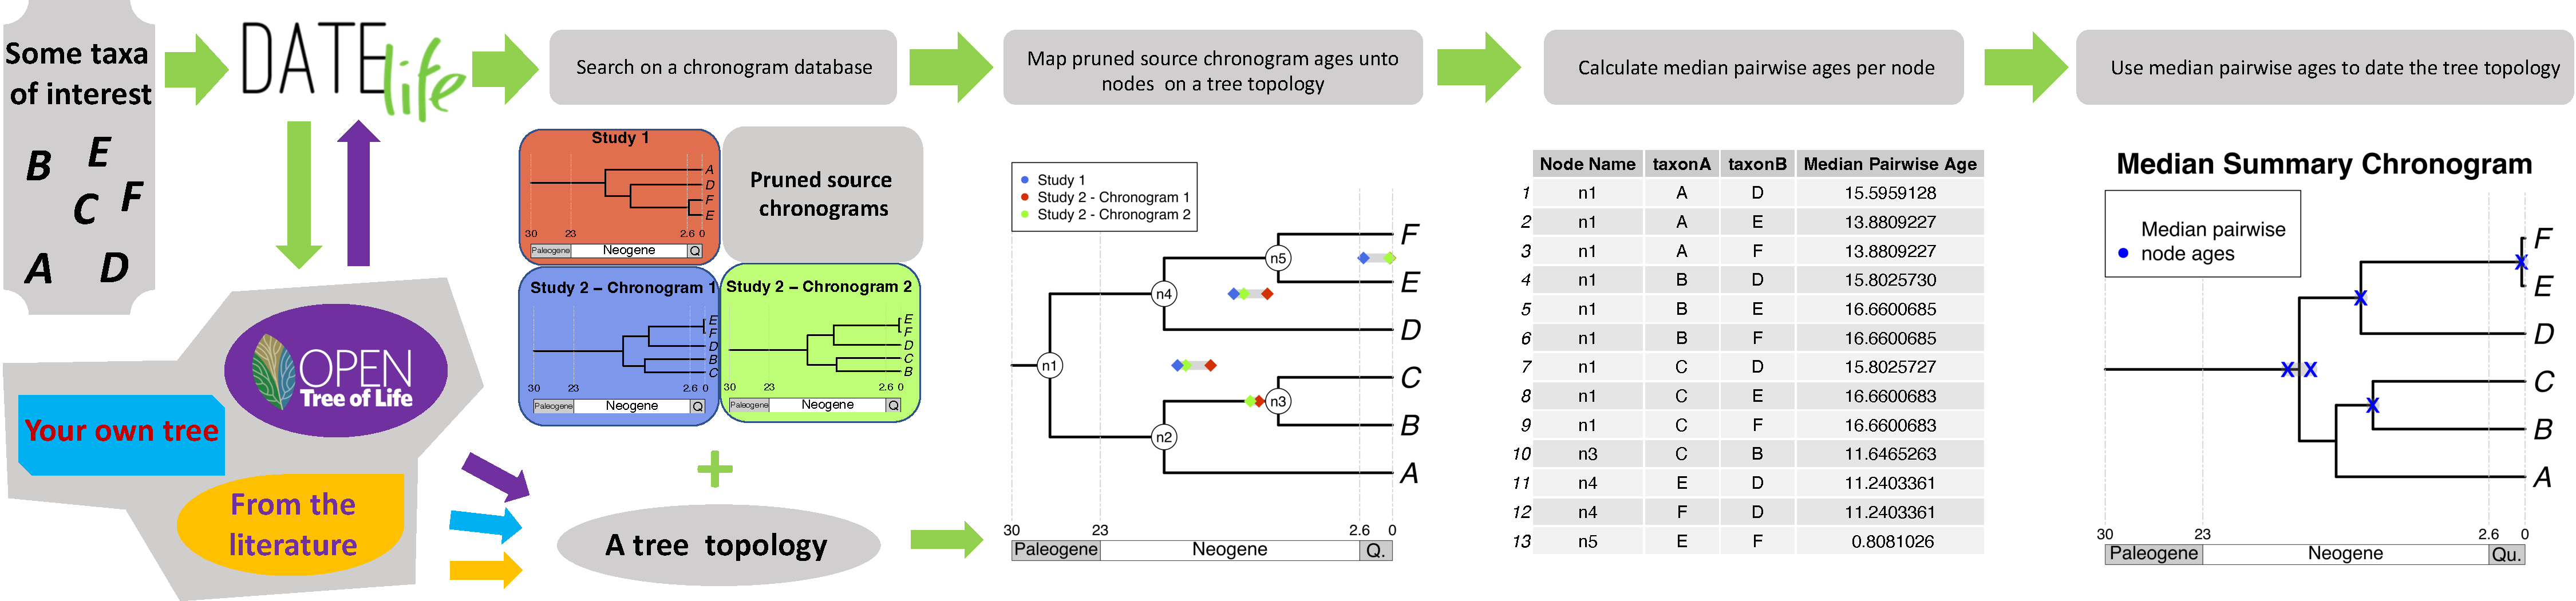
\includegraphics{../figures/figure1/figure1-horizontal.pdf}
\caption{Stylized DateLife workflow. This shows the general workflows and analyses that can be performed with \texttt{datelife}, via the R package or through the website  at \url{www.datelife.org/query/}. Details on the functions involved on each workflow are shown in \texttt{datelife}'s R package vignette.}
\label{fig:workflow}
\end{figure}
% \begin{center}
% \textsc{Figure \ref{fig:workflow}}
% \end{center}
% Stylized DateLife workflow. This shows the general workflows and analyses that can be performed with \texttt{datelife}, via the R package or through the website  at \url{http://www.datelife.org/}. Details on the functions involved on each workflow are shown in \texttt{datelife}'s R package vignette.
\newpage
\begin{figure}[!h]
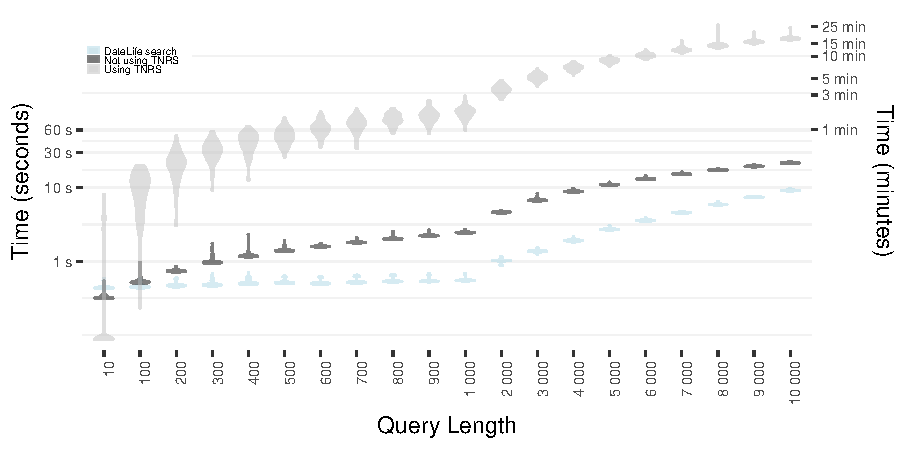
\includegraphics[width=1\linewidth]{../figures/fig_runtime_main.pdf}
\caption{Input taxon name processing and chronogram database search computation time increases with number of input taxon names. We sampled N bird species names for each input size class, 100 times, and then performed a \texttt{datelife} search using the Taxon Names Resoultion Service (TNRS; dark gray), and without using TNRS (light gray). We also performed a search using the already processed query for comparison (light blue).}
\label{fig:runtime1}
\end{figure}
% \begin{center}
% \textsc{Figure \ref{fig:runtime1}}
% \end{center}
%
\newpage
\begin{figure}[!h]
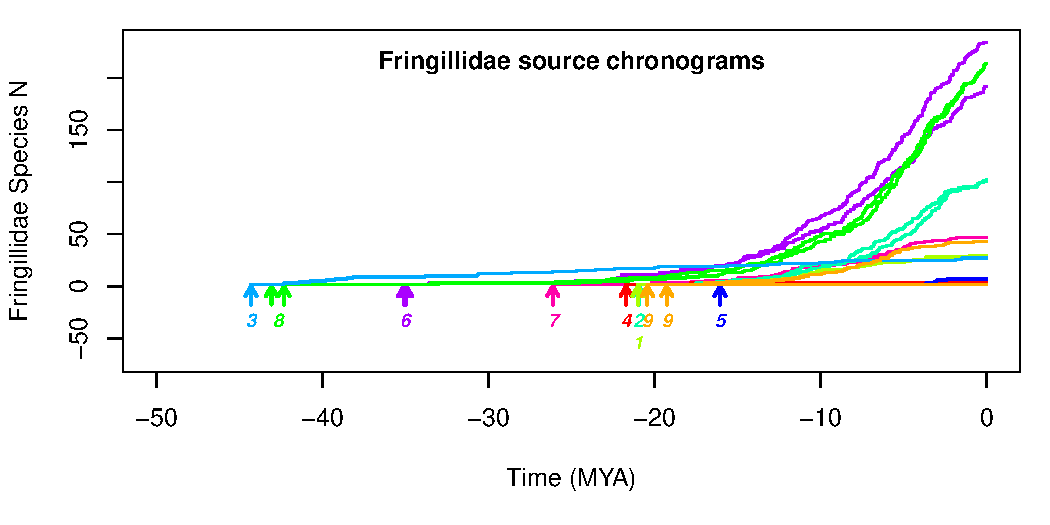
\includegraphics[width=1\linewidth]{../figures/fig_schronograms1.pdf}
\caption{Lineage through time (LTT) plots of source chronograms containing all or a subset of species from the bird family Fringillidae of true finches. Arrows indicate maximum age of each chronogram. Numbers reference to chronograms' original publications 1: Barker et al. (\protect\hyperlink{ref-barker2012going}{2012}), 2: Barker et al. (\protect\hyperlink{ref-barker2015new}{2015}), 3: Burns et al. (\protect\hyperlink{ref-burns2014phylogenetics}{2014}), 4: Claramunt and Cracraft (\protect\hyperlink{ref-claramunt2015new}{2015}), 5: Gibb et al. (\protect\hyperlink{ref-gibb2015new}{2015}), 6: Hedges et al. (\protect\hyperlink{ref-Hedges2015}{2015}), 7: Hooper and Price (\protect\hyperlink{ref-hooper2017chromosomal}{2017}), 8: Jetz et al. (\protect\hyperlink{ref-Jetz2012}{2012}), 9: Price et al. (\protect\hyperlink{ref-price2014niche}{2014}).
}
\label{fig:schronograms1}
\end{figure}
% \begin{center}
% \textsc{Figure \ref{fig:schronograms1}}
% \end{center}
%Lineage through time (LTT) plots of source chronograms containing all or a subset of species from the bird family Fringillidae of true finches. Arrows indicate maximum age of each chronogram. Numbers reference to chronograms' original publications 1: Barker et al. (\protect\hyperlink{ref-barker2012going}{2012}), 2: Barker et al. (\protect\hyperlink{ref-barker2015new}{2015}), 3: Burns et al. (\protect\hyperlink{ref-burns2014phylogenetics}{2014}), 4: Claramunt and Cracraft (\protect\hyperlink{ref-claramunt2015new}{2015}), 5: Gibb et al. (\protect\hyperlink{ref-gibb2015new}{2015}), 6: Hedges et al. (\protect\hyperlink{ref-Hedges2015}{2015}), 7: Hooper and Price (\protect\hyperlink{ref-hooper2017chromosomal}{2017}), 8: Jetz et al. (\protect\hyperlink{ref-Jetz2012}{2012}), 9: Price et al. (\protect\hyperlink{ref-price2014niche}{2014}).
\newpage
\begin{figure}[!h]
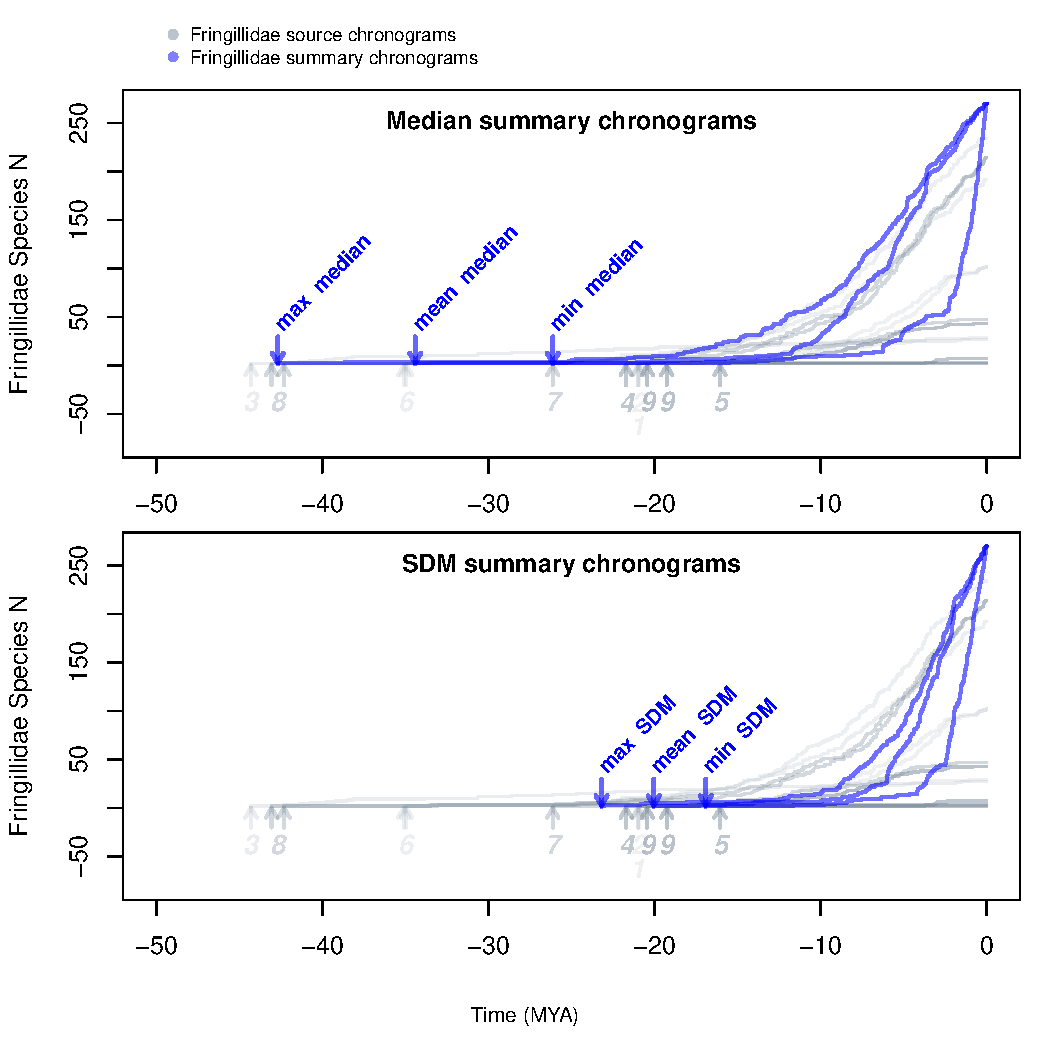
\includegraphics{../figures/fig_summaries.pdf}
\caption{LTT plots of median (top) and Supermatrix Distance Method (SDM; bottom) chronograms summarising information from source chronograms found for the Fringillidae. Arrows indicate tree maximum age.}
\label{fig:summaries}
\end{figure}
% \begin{center}
% \textsc{Figure \ref{fig:summaries}}
% \end{center}
% LTT plots of median (top) and Supermatrix Distance Method (SDM; bottom) chronograms summarising information from source chronograms found for the Fringillidae. Arrows indicate tree maximum age.
\newpage
\begin{figure}[!h]
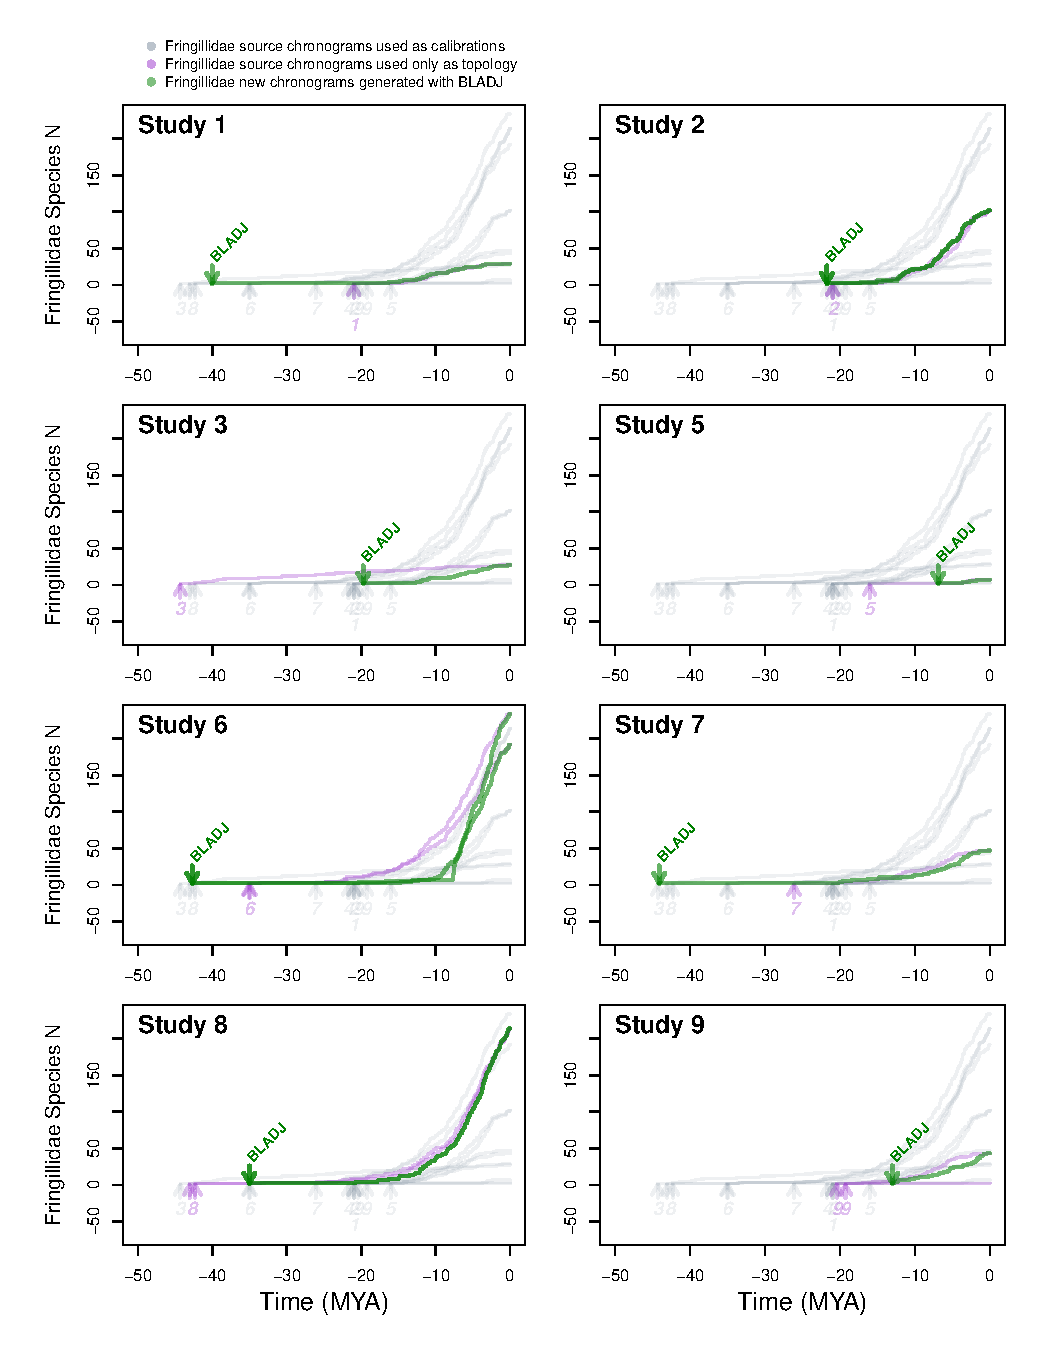
\includegraphics{../figures/fig_crossval_bladj.pdf}
\caption{LTT plots showing results from the cross-validation analyses of trees without branch lengths dated using BLADJ. The dating analysis can only be performed in trees with more than 2 tips, thus excluding chronogram from study 4; its data was still used as calibration for the other source chronograms.}
\label{fig:cvbladj}
\end{figure}
% \begin{center}
% \textsc{Figure \ref{fig:cvbladj}}
% \end{center}
% LTT plots showing results from the cross-validation analyses of trees without branch lengths dated using BLADJ. The dating analysis can only be performed in trees with more than 2 tips, thus excluding chronogram from study 4; its data was still used as calibration for the other source chronograms.
\newpage
\begin{figure}[!h]
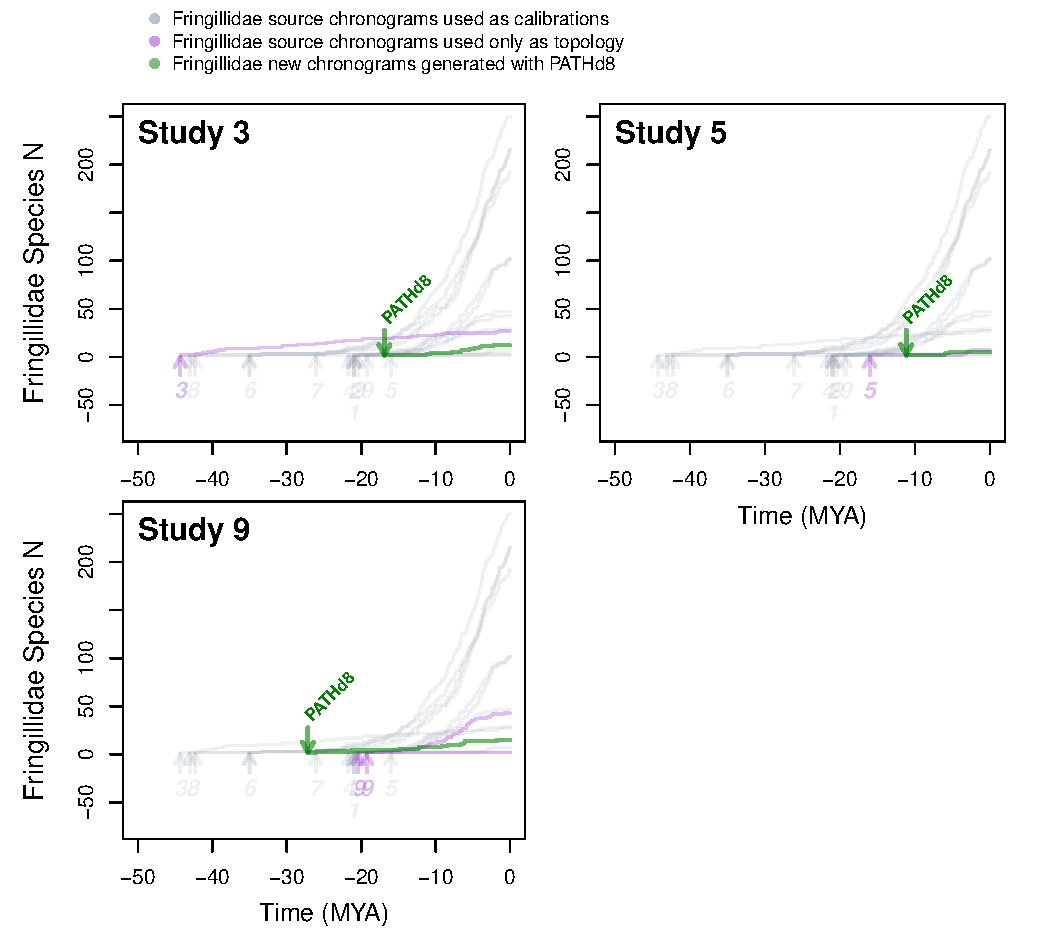
\includegraphics{../figures/fig_crossval_boldsumm.pdf}
\caption{LTT plots showing results from the cross-validation analyses of trees with branch length reconstructed with data from the Barcode of Life Database (BOLD) dated using PATHd8. We could construct a tree with branch lengths for all source chronograms. However, dating with PATHd8 was only successful in three source chronograms shown here.}
\label{fig:cvbold}
\end{figure}
% \begin{center}
% \textsc{Figure \ref{fig:cvbold}}
% \end{center}
FIGURES
%LTT plots showing results from the cross-validation analyses of trees with branch length reconstructed with data from the Barcode of Life Database (BOLD) dated using PATHd8. We could construct a tree with branch lengths for all source chronograms. However, dating with PATHd8 was only successful in three source chronograms shown here.

%\end{linenumbers}
